\documentclass[paper=a5,fontsize=9pt]{jlreq}
\usepackage{luatexja-fontspec}
\setmainfont{DejaVu Serif}[Scale=0.9]
\setmainjfont{YuKyo_Yoko-Medium}[BoldFont=YuKyo_Yoko-Bold]
\usepackage{rank-2-roots}
\usepackage[mark=o]{dynkin-diagrams}

\title{ルート系とディンキン図形}
\author{宇佐見 公輔}
\date{すうがく徒のつどい@オンライン}
\begin{document}
\maketitle

ルート系(root system)は、リー代数(Lie algebra)を分類する研究の中で現れました。

\begin{figure}
    \centering
    \scalebox{0.8}{
        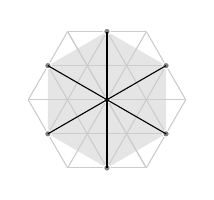
\begin{tikzpicture}
            \begin{rootSystem}{A}
                \roots
                \wt{0}{0}
                \draw \weight{0}{0} -- \weight{1}{1};
                \draw \weight{0}{0} -- \weight{-1}{-1};
                \draw \weight{0}{0} -- \weight{1}{-2};
                \draw \weight{0}{0} -- \weight{-1}{2};
                \draw \weight{0}{0} -- \weight{2}{-1};
                \draw \weight{0}{0} -- \weight{-2}{1};
            \end{rootSystem}
        \end{tikzpicture}
    }
    \scalebox{1.2}{
        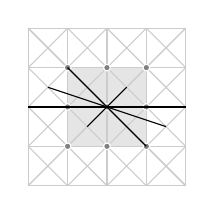
\begin{tikzpicture}
            \begin{rootSystem}{B}
                \roots
                \wt{0}{0}
                \draw \weight{0}{0} -- \weight{0}{2};
                \draw \weight{0}{0} -- \weight{0}{-2};
                \draw \weight{0}{0} -- \weight{1}{0};
                \draw \weight{0}{0} -- \weight{-1}{0};
                \draw \weight{0}{0} -- \weight{1}{-2};
                \draw \weight{0}{0} -- \weight{-1}{2};
                \draw \weight{0}{0} -- \weight{2}{-2};
                \draw \weight{0}{0} -- \weight{-2}{2};
            \end{rootSystem}
        \end{tikzpicture}
    }
\end{figure}

複素数体上の有限次元単純リー代数の分類は、ルート系の分類をすることで行えます。
ルート系の分類には、ディンキン図形(Dynkin diagram)を用います。

\begin{figure}
    \centering
    \scalebox{2}{
        \dynkin{A}{3}
    }
    \scalebox{2}{
        \dynkin{C}{5}
    }
    \scalebox{2}{
        \dynkin{D}{4}
    }
    \scalebox{2}{
        \dynkin{E}{6}
    }
    \scalebox{2}{
        \dynkin{F}{4}
    }
    \scalebox{2}{
        \dynkin{G}{2}
    }
\end{figure}

ルート系とディンキン図形は発祥はリー理論ですが、それ以外に、正多面体群、有限鏡映群、特異点、楕円曲面、パンルヴェ方程式、など様々なところで現れることが知られています。

今回は、ルート系やディンキン図形の定義や性質についてお話しします。

\end{document}
